% 1987 年全国卷文科第五题：二次函数图象
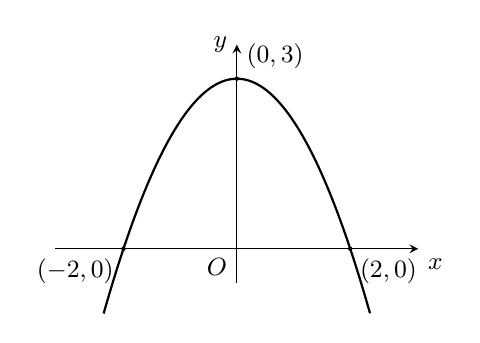
\begin{tikzpicture}[scale=0.72,>=stealth,font=\small]
  \draw[->] (-3.2,0)--(3.2,0) node[below right] {$x$};
  \draw[->] (0,-0.6)--(0,3.6) node[left] {$y$};
  \draw[thick,domain=-2.35:2.35,samples=80]
    plot (\x,{3-0.75*\x*\x});
  \fill (-2,0) circle (1.1pt) node[below left] {$(-2,0)$};
  \fill (2,0) circle (1.1pt) node[below right] {$(2,0)$};
  \fill (0,3) circle (1.1pt) node[above right] {$(0,3)$};
  \node[below left] at (0,0) {$O$};
\end{tikzpicture}
